% !TEX root = ../main.tex

\chapter{Memory Access Tracing}

\section{MAT Introduction}

In Linux, tracing memory access for tasks\footnote{In Linux Scheduler, processes and threads are often treated equally, so here we don't make clear distinction, and refer to both processes and threads as tasks.} is useful. Although the hardware uses a R bit and a M bit to track if a page has been referenced or modified, it does not maintain access frequency for each task. Therefore, we try to propose a per task memory access tracing method, which can trace the number of times a given range of memory is written by a particular task. Based on the tracing mechanism, we can use these tracing data to calculate the race probabilities between different tasks.

\section{MAT Design}

To tracing the writes of a given range of memory, we can take full advantage of the Page Fault mechanism. Firstly, invoke linux system call \textit{mprotect} on given range of memory before any writes to set the memory as Read-Only. The system call \textit{mprotect} changes the access protections for the calling task's memory pages containing any part of the given address range. If the calling task tries to access memory in a manner that violates the protections, then the kernel generates a SIGSEGV signal for the task\cite{mprotect}. Now, if we try to write to the protected memory, the kernel will send us a SIGSEGV signal. Secondly, after capturing the signal in user space, we can customize the method to deal with it. We call it the SIGSEGV handler. In the handler, we just simply invoke the \textit{mprotect} again, but this time we set the memory as Read-Write. Then we can write to the memory normally. Thirdly, in the kernel space, on the path that the kernel generates the SIGSEGV signal due to access permission error, we can perceive that in the user space a write was performing. Thus, memory access tracing is achieved.

\begin{figure}[!htp]
  \centering
  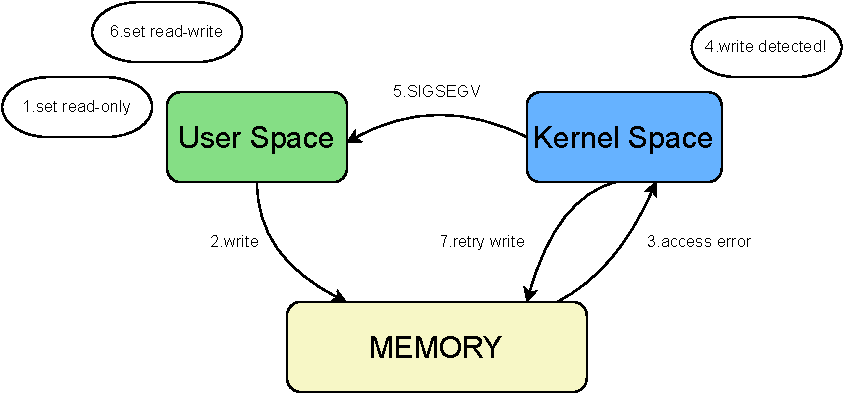
\includegraphics[width=12cm]{figures/memaccess.drawio.pdf}
  \caption{Memory Access Tracing Procedure}
\end{figure}

After the analysis above, we can find that to detect and record memory writes, we need to do some modification on the path that the kernel sends the SIGSEGV signal. If a SIGSEGV is to be generated and we are tracing the task, the kernel would add one to the write counts of the task.

\section{MAT Implementation}

To apply the memory access tracing to linux kernel, we implement three system calls. Load the three modules into the kernel, and then we can use these system calls to start tracing, stop tracing, and getting the tracing results:

\begin{itemize}
    \item \textbf{\textit{sys\_start\_trace(pid\_t pid)}}: tell the kernel to start tracing memory writes of the given pid.
    \item \textbf{\textit{sys\_stop\_trace(pid\_t pid)}}: tell the kernel to stop tracing memory writes of the given pid.
    \item \textbf{\textit{sys\_get\_trace(pid\_t pid, int *wcounts)}}: get the memory writes times of the given pid.
\end{itemize}

Besides, we add some variables to the \textit{task\_struct}\footnote{\textit{task\_struct} is a data structure in linux kernel. It records the information of a process.} to record the tracing states of the task. Finally, we add some code to the kernel on the path to send SIGSEGV. These code segments will update the write counts if we are tracing the running task.

\subsection{Task Struct}

We add a integer variable \textit{wcounts} to record the write times and a boolean variable \textit{trace\_flag} to determine when to start tracing:

\begin{codeblock}[language=C]
// include/linux/sched.h
struct task_struct {
	... 
	int wcounts; // record the write times	
	int trace_flag;	// 0 not tracing, 1 tracing
  ...
};
\end{codeblock}

\subsection{Update Write Count}

In the kernel source code of the page fault process, we add some code to update the write counts if we are tracing the task:

\begin{codeblock}[language=C]
// arch/arm/mm/fault.c
static int __kprobes
do_page_fault(unsigned long addr, unsigned int fsr, struct pt_regs *regs)
{
    ...
    if (fault & VM_FAULT_SIGBUS) {
		...
	  } else {
	    ... 
		  if (tsk->trace_flag) // SIGSEGV! If tracing, add one to task wcounts	
		  	tsk->wcounts++;
	  }
	  ...
}
\end{codeblock}

\subsection{System Calls}

In \textit{sys\_start\_trace}, we set the \textit{trace\_flag} of the task corresponding to the given pid to 1. If we have already been tracing the task, do nothing and return \textit{-EINVAL}:

\begin{codeblock}[language=C]
static int sys_start_trace(pid_t pid)
{
    struct task_struct *task;
    task = get_pid_task(find_get_pid(pid), PIDTYPE_PID); // get task by pid
    if (!task || task->trace_flag == 1)
        return -EINVAL;
    task->trace_flag = 1; // start tracing
    task->wcounts = 0;
    return 0;
}
\end{codeblock}

In \textit{sys\_stop\_trace}, we set the \textit{trace\_flag} to 0, and reset the \textit{wcounts} to 0. If we haven't traced the task yet, return \textit{-EINVAL}:

\begin{codeblock}[language=C]
static int sys_stop_trace(pid_t pid)
{
    struct task_struct *task;
    task = get_pid_task(find_get_pid(_pid), PIDTYPE_PID); // get task by pid
    if (!task || task->trace_flag == 0)
        return -EINVAL;
    task->trace_flag = 0; // stop tracing
    task->wcounts = 0;
    return 0;
}
\end{codeblock}

In \textit{sys\_get\_trace}, we get the task's \textit{wcounts}. If we haven't traced the task yet, return \textit{-EINVAL}:

\begin{codeblock}[language=C]
static int sys_get_trace(pid_t _pid, int *wcounts)
{
    struct task_struct *task;
    task = get_pid_task(find_get_pid(_pid), PIDTYPE_PID); // get task by pid
    if (!task || task->trace_flag == 0)
        return -EINVAL;
    *wcounts = task->wcounts; // get the wcounts
    return 0;
}
\end{codeblock}

\section{MAT Test}

We have written a test program to test three system calls and memory access tracing we implement. The test results are shown as following:

\begin{figure}[!htp]
\begin{minipage}{0.48\textwidth}
  \centering
  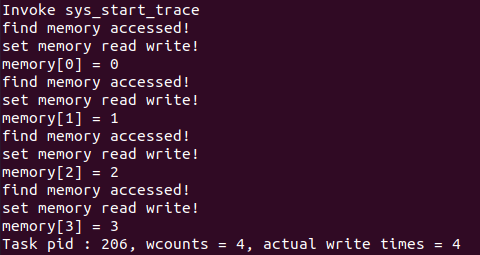
\includegraphics[height=3.8cm]{figures/mattest1.png}
  \caption{Start Tracing Test}
  \label{fig:memtest1}
\end{minipage}\hfill
\begin{minipage}{0.48\textwidth}
  \centering
  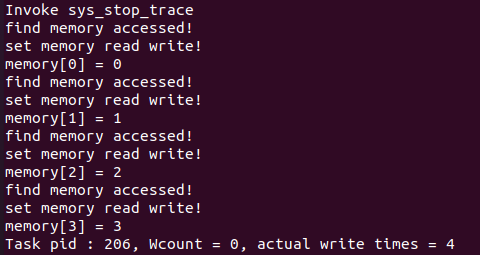
\includegraphics[height=3.8cm]{figures/mattest2.png}
  \caption{Stop Tracing Test}
  \label{fig:memtest2}
\end{minipage}
\end{figure}

In Figure~\ref{fig:memtest1} we can see that after we invoke \textit{sys\_start\_trace}, the memory access tracer can record the write times correctly. In Figure~\ref{fig:memtest2} we can see that after we invoke \textit{sys\_stop\_trace}, the kernel would stop tracing the task's memory accesses. Thus, we successfully implement the memory access tracing.

\section{MAT Conclusion}

In this project, we implemented the Memory Access Tracing and got the correct test results. Using the tracing data, we can further compute the race probabilities between different tasks. This can help us to accomplish the Race-Averse Scheduler.

However, there still exist some imperfections in our implementation. First, the tracing can not be done only by kernel. We have to use \textit{mprotect} to set protection for the memory before any write in user space. Can we set protection automatically in kernel space? If we achieve this, we can trace the memory access only by invoking \textit{sys\_start\_trace}, and perform writes without additional explicit protection in user space, which is apparently more reasonable and elegant. Second, because we borrow the page fault handler to detect the writes in kernel space, every write associated with the tracing memory will result in a page fault. Is it an acceptable overhead? If it significantly affects the write performance, we have to re-evaluate its value.
